\graphicspath{ {report_template/Images/} }
\chapter{Introduction}
The goal of this chapter is to highlight the main technologies that are used to build a modern microphone: MEMS and ECM. 
\newline
In the next chapter the watermarking procedure will be described in detail and how such technique helped to implement the use case of the project. \newline
Chapter 3 describes the state of the art of modern day attacks and then in the last chapter the implementation and the results of the project will be discussed and presented.
\section{MEMS}
MEMS (Micro-Electro-Mechanical System) Microphones use a MEMS component placed on a printed circuit board (PCB) and protected with a mechanical cover. A small hole is fabricated in the case to allow sound into the microphone and is either designated as top-ported if the hole is in the top cover or bottom-ported if the hole is in the PCB. The MEMS component is often designed with a mechanical diaphragm and mounting structure created on a semiconductor die.
\subsection{How it works}
The MEMS diaphragm forms a capacitor and sound pressure waves cause movement of the diaphragm. MEMS microphones typically contain a second semiconductor die which functions as an audio preamplifier, converting the changing capacitance of the MEMS to an electrical signal. The output of the audio preamplifier is provided to the user if an analog output signal is desired. If a digital output signal is desired, then an analog-to-digital converter (ADC) is included on the same die as the audio preamplifier. A common format used for the digital encoding in MEMS microphones is pulse density modulation (PDM), which allows for communication with only a clock and a single data line. Decoding of the digital signal at the receiver is simplified due to the single bit encoding of the data. Digital I²S outputs are a third option that include an internal decimation filter, which allows for processing to be completed in the microphone itself. This means the microphone can connect directly to a digital signal processor (DSP) or microcontroller, eliminating the need for an ADC or codec in many applications.
\begin{figure}[H]
    \centering
    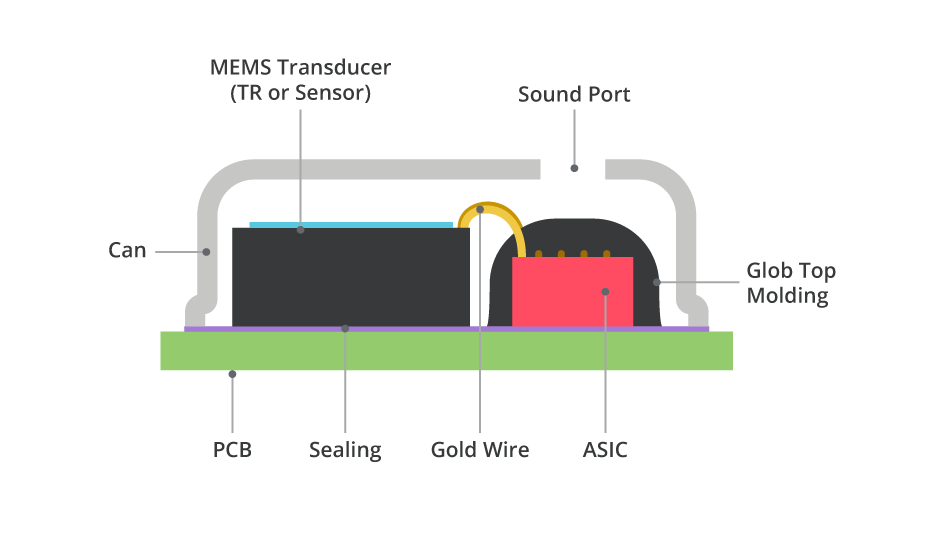
\includegraphics[width=8cm]{report_template/images/MEMS.png}
    \caption{: MEMS Structure}
    \label{fig:MEMS}
\end{figure}

\subsection{ECM}
An electret diaphragm (material with a fixed surface charge) is spaced close to a conductive plate, and similar to MEMS microphones, a capacitor is formed with the air gap as the dielectric. Voltage across the capacitor varies as the value of the capacitance changes due to sound pressure waves moving the electret diaphragm, $\Delta$V = Q/ $\Delta$C. The capacitor voltage variations are amplified and buffered by a JFET internal to the microphone housing. The JFET is typically configured in a common-source configuration, while an external load resistor and dc blocking capacitor are used in the external application circuit.
\break
\begin{figure}[H]
    \centering
    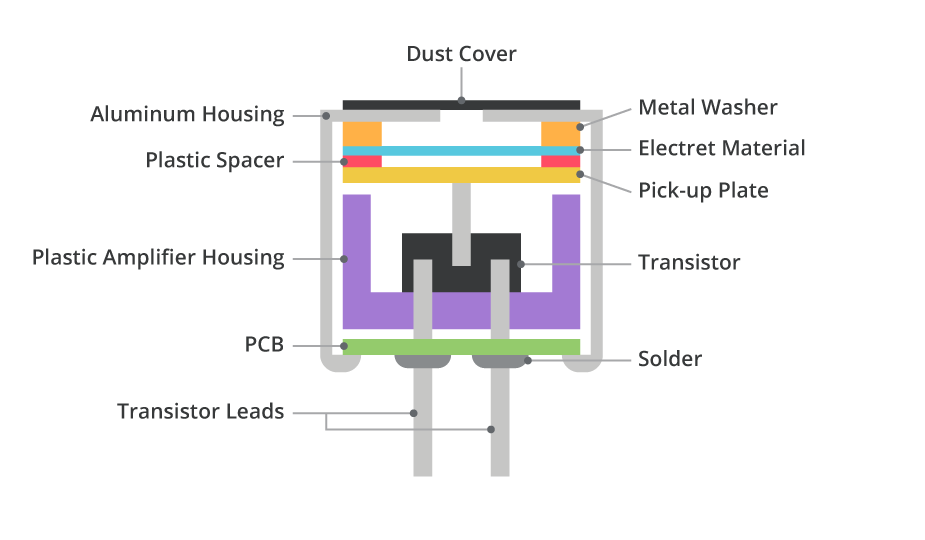
\includegraphics[width=8cm]{report_template/images/ECM.png}
    \caption{: ECM Structure}
    \label{fig:ECM}
\end{figure}
\section{Main differences}
Due to their small size, electrical noise immunity, and mechanical robustness, MEMS microphones are becoming increasingly popular. However, this does not mean that they are the de-facto best choice for every application. Many legacy applications may benefit from a simple change or upgrade to their current ECM. Apart from their excellent IP ratings, which allow them to perform well in harsh environments, the intrinsic nature of ECMs also makes them an excellent choice for applications that benefit from noise-canceling or unidirectionality.
\newpage
If the space constraints placed upon a design are particularly acute (such as in smartphones, wearables, hearing aid implants, etc.), or there is likely to be the need to distribute multiple microphones throughout an item of equipment (like in a VR headset for instance) then MEMS may be the better option.
Conversely, if elevated performance or resilience to challenging operating conditions are a priority, then ECM could prove to be the more appropriate route to take. Therefore, professional audio equipment, voice-controlled home assistants, voice recognition systems, and a wide range of other applications will continue to rely on these devices.
\newline
\newline
In our project we wanted to focus on common devices like smartphones, therefore we decided to develop solutions working on MEMS microphones.
 During the last decade the usage of MEMS in common devices raised significatively (back in 2009 when Apple started to use MEMS microphones for iPhone 4) and since the project focused on such devices like smartphones due to the nature of the attack and the target of the attacks, the solution that has been implemented was on MEMS microphones.
 As shown in Figure 1.3 it is possible to understand why it is much more useful for the purpose of this project to consider MEMS technology rather then the ECM, it is sufficient to consider Average Growth Rate to take into account the rising of the first technology and the falling of the latter
 .
\newline
 \begin{figure}[H]
    \centering
    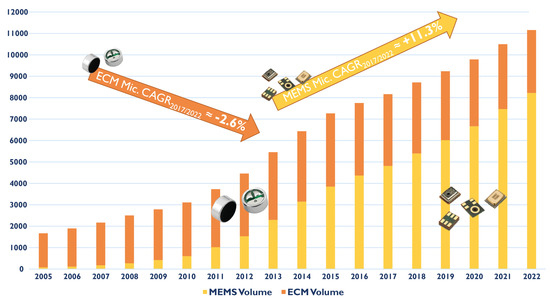
\includegraphics[width=10cm]{report_template/images/market.jpg}
    \caption{: Market Evolution}
    \label{fig:market}
\end{figure}
\section{Exploiting Non-Linearity in MEMS microphones}
Even though this effect is not exploited unless very high frequencies (order of 60kHz) are used it is really important to describe one of the core development of this project: the nonlinearity of this technology.

Modules inside a microphone are mostly linear systems, in the case of the pre-amplifier with input S:
\[ S_{out} = A_1S\]
Acoustic amplifiers maintain a strong linearity only in the audible frequency range but outside of this range the response exhibits non linearity. Thus, for f $>$ 25kHz, the net recorded $S_{out}$ can be expressed as:
\[S_{out}\Bigg|_{f>25} = \sum_{i=1}^{\infty}A_iS^i=A_1S+A_2S^2+A_3S^3+...\]
With the third and higher terms that are extremely weak and can be ignored.
\newpage
To operate the microphone in its non-linear range, one can play a sound S composed of two tones S$_1$ = 40 and S$_2$ = 50 kHz.
S = $Sin(2\pi40t)+Sin(2\pi50t)$.
After passing through the diaphragm and pre-amplifier of the microphone, the output $S_{out}$ can be modeled as:
\[S_{out}= A_1(S_1 + S_2) + A_2(S_1 + S_2)^2 =\] \[ = A_1[Sin(\omega_1t) + Sin(\omega_2t)] + A_2 [Sin^2(\omega_1t) + Sin^2(\omega_2t) + 2Sin(\omega_1t)Sin(\omega_2t)\]
where $\omega_1$ = 2$\pi$40 and $\omega_2$ = 2$\pi$50.
\newline
The first order terms produce frequencies out of the microphone's cutoff, the second order term  instead is a multiplication of signals, resulting in different frequencies for each component such as 2$\omega_1$, 2$\omega_2$, ($\omega_1$ - $\omega_2$) and ($\omega_1$ + $\omega_2$). Mathematically, 
\[ A_2(S_1 + S_2)^2 = 1 - \frac{1}{2}Cos(2\omega_1t) - \frac{1}{2}Cos(2\omega_2t) + Cos((\omega_1 - \omega_2)t) - Cos((\omega_1 + \omega_2)t)\]
With the cutoff frequency at 24kHz, every frequency gets filtered except for the $\omega_1 - \omega_2$ component, that results in a 10kHz tone, this allows a totally inaudible frequency to be recorded by the microphone.
This is the main concept that revolves around this project and some possible future implementations and improvements. \cite{backdoor}
\newline
The goal of the project proposed is to show how some high frequency tones can carry some data thanks to Watermarking, anyway if the data can be carried at such high frequency the future improvement can basically carry these information at an even higher frequency thanks to the implementation of an amplifier and work at inaudible frequencies.
\newline
 \begin{figure}[H]
    \centering
    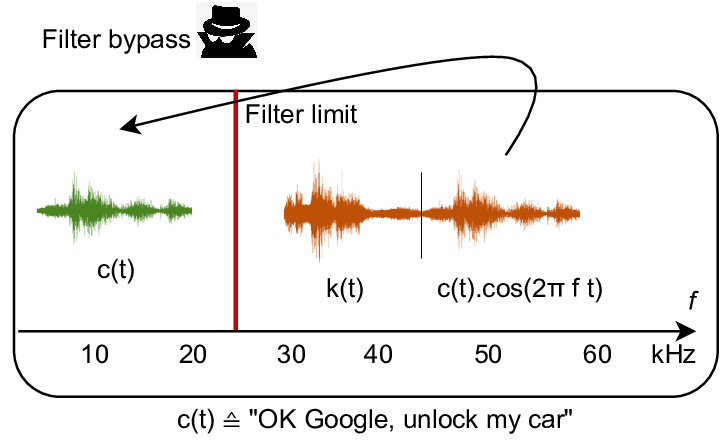
\includegraphics[width=10cm]{report_template/images/Bypass.png}
    \caption{: Example of a filter bypass exploiting non linearity}
    \label{fig:market}
\end{figure}

\newpage
You can cite references like this: \cite{texbook} \cite{lamport94}, by using the \lstinline{\cite} directive. You have to copy within \lstinline{\cite} brackets the label of the entry that you have in the BibTeX file (\texttt{.bib}). The \texttt{.bib} file of this thesis is \texttt{mybib.bib}. he command \lstinline{\addbibresource} at the top of this main file indicates what BibTeX file you are referring to.

As an example, this is a BibTeX entry:

\begin{verbatim}
@inproceedings{urias2018cyber,
  title={Cyber Range Infrastructure Limitations and Needs of Tomorrow: A Position Paper},
  author={Urias, Vincent E and Stout, William MS and Van Leeuwen, Brian and Lin, Han},
  booktitle={2018 International Carnahan Conference on Security Technology (ICCST)},
  pages={1--5},
  year={2018},
  organization={IEEE}
}
\end{verbatim}

For every online paper that you may read on online libraries, you can download its BibTeX entry. For example:
\begin{enumerate}
	\item For IEEE Xplore, click on the paper name, then click on ``Cite This'', ``BibTeX'', and you can find the entry;
	\item For Google Scholar, click on the ``Cite'' voice under the paper name, then click ``BibTeX'', and you can find the entry.
\end{enumerate}

Just copy and paste such an entry in the .bib file. If you find a paper on Scholar that is nevertheless published by IEEE, by convention you should take the entry from the IEEE website and not from Scholar. To do this, just click on the title of the paper. This will redirect you to the resource page on IEEE Xplore. Once here, follow instructions at point 1.

When you compile, a correct number will automatically be assigned to the citation in the text, and the complete entry will appear at the bottom of the document, in the ``Bibliography'' chapter.

If you need to cite a generic online resource, which does not necessarily correspond to a scientific paper, use the \lstinline{@misc} entry in the \texttt{.bib} file. A \lstinline{@misc} entry looks like this:

\begin{verbatim}
@misc{nist2018,
    author = "{NIST}",
    title = "Cyber Ranges",
    year = "2018",
    howpublished = "\url{https://www.nist.gov/system/files/documents/2018/02/13/cyber_ranges.pdf}",
    note = "[Online; Accessed 2019, 28 November]"
  }
\end{verbatim}

You have to manually create this entry from scratch and manually type these fields. Remember not to forget any of these fields. You can choose the label with which to refer to the resource. The title of the website (which you can see at the top of the tab of your browser showing the page) can be used as the title of the resource.

In general, enter a citation of this type for sites only when there are data, phrases, or images that you intend to report. Instead, if you want to cite names of software or hardware devices, prefer the use of the \lstinline{\footnote}, in which you will only have to specify the URL of the item.

Remember that citations, both in the text and in the image captions, usually go to the end of a sentence, before the fullstop, as in this case \cite{vykopal2017kypo}. In case of long periods, they can also be placed before other detachment signs, such as commas or semicolons, or colons if they precede a list, itemized or enumerated. An exemption is allowed in the event that the name of research projects, described in some scientific resource, is being introduced, as in this case:

\begin{center}
	Cybertropolis \cite{deckard2018cybertropolis} is described in a very good paper by Gary Deckard.
\end{center}

Remember to put citations very often to justify your claims, especially when you report data or results. Just consider them as a justification of what you, in an original way, are writing. Citations are not needed to have permission to copy and paste sentences from online resources, which should NEVER be done - always try to rephrase the concept with your words.

\begin{figure}[h!]
	\vspace{0.5cm}
	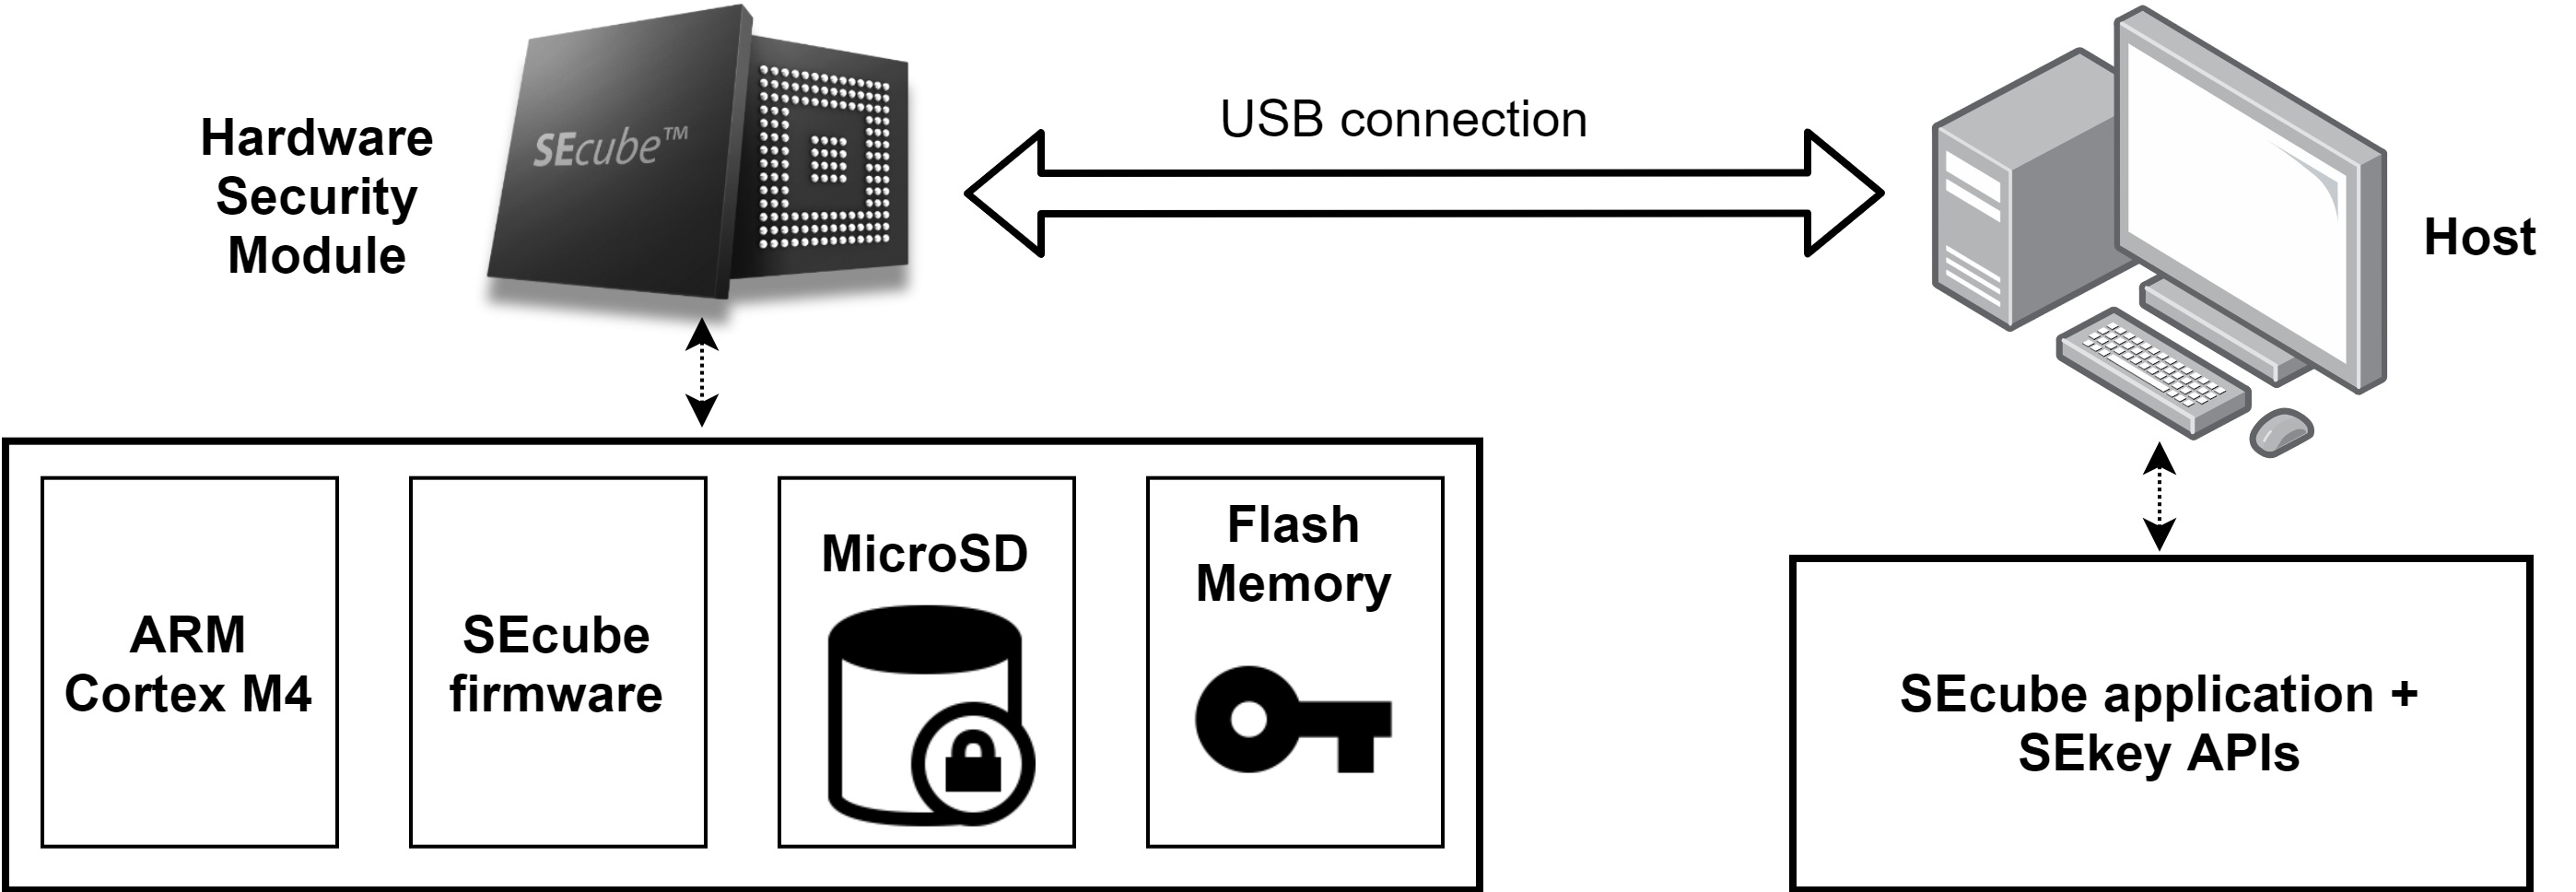
\includegraphics[width=\textwidth]{images/simplearch.jpg}
	\caption{This is the image \emph{caption}.}
	\label{fig:generalschema} % This is the image label, with which you can refer to the image in any document location.
\end{figure}

This is an image example. Images must ALWAYS be understandable: never introduce images that have text smaller than the text in your document. If you create the images yourself, try not to make them clash too much with the style of your document, and use the same font as this thesis.
If they are not images of your own creation, you MUST reference them. In the caption of the image, you need to insert a citation to the resource from which you took the image, at the end of the caption sentence, before the fullstop.
Each image you enter MUST be referenced in the text, using a formula similar to this:

\begin{center}
	Figure \ref{fig:generalschema} describes the architecture of the system.
\end{center}

You can refer to the image using \lstinline{\ref} followed by the image label, that you put in the \lstinline{\label} entry of the figure. Remember to use the word Figure with a capital F.

Remember that the more your text is adorned with figures, the more understandable, appreciable and readable it becomes.

\section{Section title}\label{examplesection}
This is a section under a chapter. The number of sections also contributes to greater readability of your text, and to a better display of the content in the index. In fact, sections are automatically shown in the Table of Contents. However, try not to make sections shorter than two pages. For smaller portions of your text, use subsections.

You can refer to a section using its label, using the \lstinline{\ref} directive as for images, like this:

\begin{center}
	This concept has been explained in Section \ref{examplesection}.
\end{center}

Remember to use the word Section with a capital S. This is also valid for chapters.

\subsection{Subsection title}
This is a subsection under the section.

The following is a table.

\begin{table}
	\centering
	\caption{Preliminary Experimental Results}
	\begin{tabular}{| p{3cm} | p{3cm} | p{3cm} |}
		\hline
		\textbf{Benchmark} & \textbf{Inputs}                   & \textbf{Processing time} \\ \hline
		SHA                & Message of 100 KB                 & 368449 s                 \\ \hline
		RIJNDAEL           & Message of 100 KB                 & 1083568 s                \\ \hline
		DIJKSTRA           & Matrix of 100x100 32-bit integers & 324782 s                 \\ \hline
		STRING             & 1331 50-char strings              & 178616 s                 \\ \hline
		BITCOUNT           & 12800 32-bit integers             & 419545 s                 \\ \hline
		\hline
	\end{tabular}
	\label{tab:ar}
\end{table}

If you want to write a formula, you can do like this:

\begin{equation}\label{eq:thiseq}
	X_{k}=\sum _{n=0}^{N-1}x_{n}e^{-ik{\frac {2\pi }{N}}n}\quad \quad k=0,\dots ,N-1
\end{equation}

Tables and formulas are extensively documented online, and any doubts about their syntax can be easily resolved with a simple search. As for figures and sections, the same rules also apply to tables and formulas: mandatory reference in the text, possibility to use \lstinline{\label} to label them, and naming with capital letter (e.g., ``as in Table \ref{tab:ar}, as in Formula \ref{eq:thiseq}).

The following is a piece of code:

\begin{lstlisting}
int func(int N, int M) {
  float (*p)[N][M] = malloc(sizeof *p);
  if (!p)
    return -1;
  for (int i = 0; i < N; i++)
    for (int j = 0; j < M; j++)
      (*p)[i][j] = i + j;
  print_array(N, M, p);
  free(p);
  return 1;
}
\end{lstlisting}

You can customize the style of your code, changing the language, the colors of keywords, of comments or the background by changing the settings inside the \lstinline{\lstset} directive found in the main file. Usually, the listings are not referenced within the text as happens for figures, tables, formulas and sections. Do not overdo the code within your text: use it only for short passages (e.g., function prototypes, or 2 to 5 lines of code within a function to help the reader in better understanding the meaning of the text).

You can also write in-text code using the \lstinline{\lstinline} directive, \\
like this: \lstinline{int main(int argc, char** argv);}.



